% This is the Reed College LaTeX thesis template. Most of the work
% for the document class was done by Sam Noble (SN), as well as this
% template. Later comments etc. by Ben Salzberg (BTS). Additional
% restructuring and APA support by Jess Youngberg (JY).
% Your comments and suggestions are more than welcome; please email
% them to cus@reed.edu
%
% See https://www.reed.edu/cis/help/LaTeX/index.html for help. There are a
% great bunch of help pages there, with notes on
% getting started, bibtex, etc. Go there and read it if you're not
% already familiar with LaTeX.
%
% Any line that starts with a percent symbol is a comment.
% They won't show up in the document, and are useful for notes
% to yourself and explaining commands.
% Commenting also removes a line from the document;
% very handy for troubleshooting problems. -BTS

% As far as I know, this follows the requirements laid out in
% the 2002-2003 Senior Handbook. Ask a librarian to check the
% document before binding. -SN

%%
%% Preamble
%%
% \documentclass{<something>} must begin each LaTeX document
\documentclass[12pt,twoside]{reedthesis}
% Packages are extensions to the basic LaTeX functions. Whatever you
% want to typeset, there is probably a package out there for it.
% Chemistry (chemtex), screenplays, you name it.
% Check out CTAN to see: https://www.ctan.org/
%%
\usepackage{graphicx,latexsym}
\usepackage{amsmath}
\usepackage{amssymb,amsthm}
\usepackage{longtable,booktabs,setspace}
\usepackage{chemarr} %% Useful for one reaction arrow, useless if you're not a chem major
\usepackage[hyphens]{url}
% Added by CII
\usepackage{hyperref}
\usepackage{lmodern}
\usepackage{float}
\floatplacement{figure}{H}
% Thanks, @Xyv
\usepackage{calc}
% End of CII addition
\usepackage{rotating}

% Next line commented out by CII
%%% \usepackage{natbib}
% Comment out the natbib line above and uncomment the following two lines to use the new
% biblatex-chicago style, for Chicago A. Also make some changes at the end where the
% bibliography is included.
%\usepackage{biblatex-chicago}
%\bibliography{thesis}


% Added by CII (Thanks, Hadley!)
% Use ref for internal links
\renewcommand{\hyperref}[2][???]{\autoref{#1}}
\def\chapterautorefname{Chapter}
\def\sectionautorefname{Section}
\def\subsectionautorefname{Subsection}
% End of CII addition

% Added by CII
\usepackage{caption}
\captionsetup{width=5in}
% End of CII addition

% \usepackage{times} % other fonts are available like times, bookman, charter, palatino

% Syntax highlighting #22
  \usepackage{color}
  \usepackage{fancyvrb}
  \newcommand{\VerbBar}{|}
  \newcommand{\VERB}{\Verb[commandchars=\\\{\}]}
  \DefineVerbatimEnvironment{Highlighting}{Verbatim}{commandchars=\\\{\}}
  % Add ',fontsize=\small' for more characters per line
  \usepackage{framed}
  \definecolor{shadecolor}{RGB}{248,248,248}
  \newenvironment{Shaded}{\begin{snugshade}}{\end{snugshade}}
  \newcommand{\AlertTok}[1]{\textcolor[rgb]{0.94,0.16,0.16}{#1}}
  \newcommand{\AnnotationTok}[1]{\textcolor[rgb]{0.56,0.35,0.01}{\textbf{\textit{#1}}}}
  \newcommand{\AttributeTok}[1]{\textcolor[rgb]{0.77,0.63,0.00}{#1}}
  \newcommand{\BaseNTok}[1]{\textcolor[rgb]{0.00,0.00,0.81}{#1}}
  \newcommand{\BuiltInTok}[1]{#1}
  \newcommand{\CharTok}[1]{\textcolor[rgb]{0.31,0.60,0.02}{#1}}
  \newcommand{\CommentTok}[1]{\textcolor[rgb]{0.56,0.35,0.01}{\textit{#1}}}
  \newcommand{\CommentVarTok}[1]{\textcolor[rgb]{0.56,0.35,0.01}{\textbf{\textit{#1}}}}
  \newcommand{\ConstantTok}[1]{\textcolor[rgb]{0.00,0.00,0.00}{#1}}
  \newcommand{\ControlFlowTok}[1]{\textcolor[rgb]{0.13,0.29,0.53}{\textbf{#1}}}
  \newcommand{\DataTypeTok}[1]{\textcolor[rgb]{0.13,0.29,0.53}{#1}}
  \newcommand{\DecValTok}[1]{\textcolor[rgb]{0.00,0.00,0.81}{#1}}
  \newcommand{\DocumentationTok}[1]{\textcolor[rgb]{0.56,0.35,0.01}{\textbf{\textit{#1}}}}
  \newcommand{\ErrorTok}[1]{\textcolor[rgb]{0.64,0.00,0.00}{\textbf{#1}}}
  \newcommand{\ExtensionTok}[1]{#1}
  \newcommand{\FloatTok}[1]{\textcolor[rgb]{0.00,0.00,0.81}{#1}}
  \newcommand{\FunctionTok}[1]{\textcolor[rgb]{0.00,0.00,0.00}{#1}}
  \newcommand{\ImportTok}[1]{#1}
  \newcommand{\InformationTok}[1]{\textcolor[rgb]{0.56,0.35,0.01}{\textbf{\textit{#1}}}}
  \newcommand{\KeywordTok}[1]{\textcolor[rgb]{0.13,0.29,0.53}{\textbf{#1}}}
  \newcommand{\NormalTok}[1]{#1}
  \newcommand{\OperatorTok}[1]{\textcolor[rgb]{0.81,0.36,0.00}{\textbf{#1}}}
  \newcommand{\OtherTok}[1]{\textcolor[rgb]{0.56,0.35,0.01}{#1}}
  \newcommand{\PreprocessorTok}[1]{\textcolor[rgb]{0.56,0.35,0.01}{\textit{#1}}}
  \newcommand{\RegionMarkerTok}[1]{#1}
  \newcommand{\SpecialCharTok}[1]{\textcolor[rgb]{0.00,0.00,0.00}{#1}}
  \newcommand{\SpecialStringTok}[1]{\textcolor[rgb]{0.31,0.60,0.02}{#1}}
  \newcommand{\StringTok}[1]{\textcolor[rgb]{0.31,0.60,0.02}{#1}}
  \newcommand{\VariableTok}[1]{\textcolor[rgb]{0.00,0.00,0.00}{#1}}
  \newcommand{\VerbatimStringTok}[1]{\textcolor[rgb]{0.31,0.60,0.02}{#1}}
  \newcommand{\WarningTok}[1]{\textcolor[rgb]{0.56,0.35,0.01}{\textbf{\textit{#1}}}}

% To pass between YAML and LaTeX the dollar signs are added by CII
\title{Utilización de datos satelitales para la evaluación y mejora de los pronósticos numéricos en alta resolución a muy corto plazo}
\author{Paola Corrales}
% The month and year that you submit your FINAL draft TO THE LIBRARY (May or December)
\date{Algún momento de marzo 2023?}
\division{Facultad de Ciencias Exactas y Naturales}
\advisor{Victoria Galligani}
\institution{Universidad de Buenos Aires}
\degree{Tesis presentada para optar al título de Doctor de la Universidad de Buenos Aires en el área de Ciencias de la Atmósfera y los Oceanos}
%If you have two advisors for some reason, you can use the following
% Uncommented out by CII
\altadvisor{Juan Ruiz}
% End of CII addition

%%% Remember to use the correct department!
\department{Departamento de Ciencias de la Atmósfera y los Oceanos}
% if you're writing a thesis in an interdisciplinary major,
% uncomment the line below and change the text as appropriate.
% check the Senior Handbook if unsure.
%\thedivisionof{The Established Interdisciplinary Committee for}
% if you want the approval page to say "Approved for the Committee",
% uncomment the next line
%\approvedforthe{Committee}

% Added by CII
%%% Copied from knitr
%% maxwidth is the original width if it's less than linewidth
%% otherwise use linewidth (to make sure the graphics do not exceed the margin)
\makeatletter
\def\maxwidth{ %
  \ifdim\Gin@nat@width>\linewidth
    \linewidth
  \else
    \Gin@nat@width
  \fi
}
\makeatother

% From {rticles}

\renewcommand{\contentsname}{Table of Contents}
% End of CII addition

\setlength{\parskip}{0pt}

% Added by CII

\providecommand{\tightlist}{%
  \setlength{\itemsep}{0pt}\setlength{\parskip}{0pt}}

\Acknowledgements{
I want to thank a few people.
}

\Dedication{
You can have a dedication here if you wish.
}

\Preface{
This is an example of a thesis setup to use the reed thesis document class
(for LaTeX) and the R bookdown package, in general.
}

\Abstract{
The preface pretty much says it all.

\par

Second paragraph of abstract starts here.
}

	\usepackage{setspace}\onehalfspacing
% End of CII addition
%%
%% End Preamble
%%
%
\begin{document}

% Everything below added by CII
  \maketitle

\frontmatter % this stuff will be roman-numbered
\pagestyle{empty} % this removes page numbers from the frontmatter
  \begin{acknowledgements}
    I want to thank a few people.
  \end{acknowledgements}
  \begin{preface}
    This is an example of a thesis setup to use the reed thesis document class
    (for LaTeX) and the R bookdown package, in general.
  \end{preface}
  \hypersetup{linkcolor=black}
  \setcounter{secnumdepth}{2}
  \setcounter{tocdepth}{2}
  \tableofcontents

  \listoftables

  \listoffigures
  \begin{abstract}
    The preface pretty much says it all.
    
    \par
    
    Second paragraph of abstract starts here.
  \end{abstract}
  \begin{dedication}
    You can have a dedication here if you wish.
  \end{dedication}
\mainmatter % here the regular arabic numbering starts
\pagestyle{fancyplain} % turns page numbering back on
\begin{Shaded}
\begin{Highlighting}[]
\NormalTok{knitr}\OperatorTok{::}\NormalTok{opts_chunk}\OperatorTok{$}\KeywordTok{set}\NormalTok{(}
    \DataTypeTok{echo =} \OtherTok{FALSE}\NormalTok{,}
    \DataTypeTok{message =} \OtherTok{FALSE}\NormalTok{,}
    \DataTypeTok{warning =} \OtherTok{FALSE}
\NormalTok{)}
\KeywordTok{library}\NormalTok{(here)}
\end{Highlighting}
\end{Shaded}
\begin{verbatim}
here() starts at /home/paola.corrales/tesis_doctorado
\end{verbatim}
\hypertarget{introducciuxf3n}{%
\chapter*{Introducción}\label{introducciuxf3n}}
\addcontentsline{toc}{chapter}{Introducción}

\hypertarget{pronostico-de-eventos-severos}{%
\section{Pronostico de eventos severos}\label{pronostico-de-eventos-severos}}

La simulación numérica de la atmósfera, es decir, la integración de las ecuaciones que rigen la evolución del sistema atmósferico es la base para la predicción del tiempo en diversas escalas temporales desde horas a semanas.

La predicción de fenómenos meteorológicos extremos es de particular importancia ya que pueden producir cuantiosas pérdidas humanas y materiales. En Argentina, una gran cantidad de estos fenómenos están asociados a la ocurrencia de convección profunda entre los que se cuentan tornados, ráfagas intensas, precipitaciones extremas en cortos períodos de tiempo, granizo de gran tamaño y actividad eléctrica. Es por tal motivo necesario avanzar en el conocimiento de estos fenómenos y en la capacidad de pronosticar la ocurrencia de los mismos.

Si se cuenta con condiciones de borde apropiadas, es decir, una correcta representación de las características de la superficie terrestre y el tope de la atmósfera, la integración de un modelo atmosférico es un problema de condiciones iniciales. La generación de pronósticos de calidad dependerá entonces, de la capacidad del modelo para representar los procesos atmosféricos y la exactitud de las condiciones iniciales usadas (Kalnay, 2002).

El pronóstico de los fenómenos severos es a su vez un desafío científico y tecnológico muy complejo debido a la predictibilidad limitada en la mesoescala y debido a la dificultad de conocer o diagnosticar el estado de la atmósfera en escalas espaciales pequeñas y tiempos cortos (por ejemplo de 1 a 10 km y del orden de los minutos).

Uno de los métodos que pueden utilizarse para el pronóstico de fenómenos meteorológicos severos es la utilización de modelos numéricos de la atmósfera que resuelvan explícitamente la convección profunda. Diversos estudios, han comprobado que estos modelos agregan valor al pronóstico a corto plazo y que en muchos casos proveen información sobre el modo de organización de las celdas convectivas y su intensidad (Aksoy, Dowell, \& Snyder, 2010; Stensrud et al., 2013). No obstante, la capacidad de los modelos numéricos en anticipar la ubicación y tiempo de ocurrencia de eventos extremos asociados a convección es muy limitada si no se cuenta con una detallada información sobre el estado de la atmósfera en la escala de las tormentas en el momento en el que se inicializan los pronósticos numéricos (Clark, Gallus, Xue, \& Kong, 2009).

\hypertarget{asimilaciuxf3n-de-datos-como-posible-soluciuxf3n}{%
\section{Asimilación de datos como posible solución}\label{asimilaciuxf3n-de-datos-como-posible-soluciuxf3n}}

Por otro lado es posible aplicar técnicas de asimilación de datos para generar una mejor estimación de las condiciones iniciales necesarias para integrar un modelo numérico. La asimilación de datos combina de manera optima un pronóstico numérico o campo preliminar en un tiempo t con las observaciones disponibles para ese mismo tiempo, generando un análisis. Esta combinación optima toma en cuenta el error asociado a al modelo meteorológico (errores de pronóstico) y el error de las observaciones (instrumental, de representatividad) y si ambos tienen una distribución Gaussiana, el error resultante será menor a los errores originales. Por esta razón el análisis es considerado la \emph{mejor aproximación} disponible del estado real de la atmósfera.


\begin{figure}

{\centering 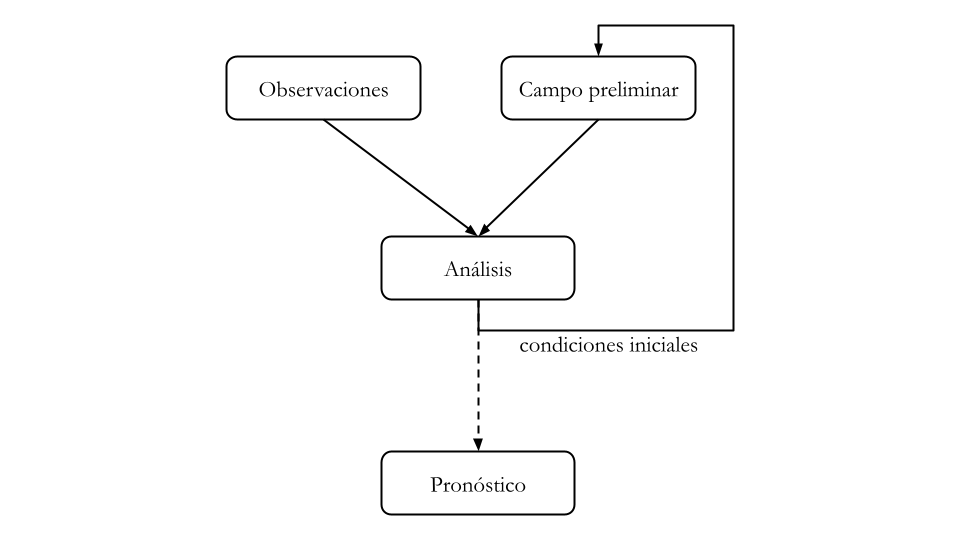
\includegraphics[width=1\linewidth]{/home/paola.corrales/tesis_doctorado/figure/ciclo_asimilacion_teorico} 

}

\caption{Esquema de un ciclo de asimilación típico. El tiempo de las observaciones y el campo preliminar deberá coincidir.}\label{fig:ciclo-asimilacion-teorico}
\end{figure}
En el caso de modelos globales, típicamente cada ciclo de asimilación de 6 horas utiliza el campo preliminar previo, es decir el pronóstico a 6 horas inicializado a partir del análisis anterior y las observaciones disponibles para las 6 horas previas o en un periodo similar centrado en la hora del análisis.
Para poder comparar el campo preliminar con las observaciones, este es interpolado a la ubicación de las observaciones. En determinados casos, por ejemplo cuando se trabaja con observaciones de satélite o radar), será necesario transformar las variables del modelo para obtener las variables observadas. En la siguiente ecuación \(H\) es el operador de las observaciones que se encarga de las interpolaciones y transformaciones necesarias sobre el campo preliminar \(x_b\).

\[ x_a = x_b + W[y_o - H(x_b )] \]
La diferencia entre las observaciones \(y_o\) y el campo preliminar se denomina innovación. El análisi \(x_a\) se obtiene aplicando las innovaciones al campo preliminar teniendo en cuenta un peso \(W\) que incluye información sobre los errores del pronóstico y de las observaciones.

Existen diferentes metodologías para obtener \(x_a\). Los métodos variacionales, 3D-Var y 4D-Var, definen una función de costo que es proporcial a la distrancia entre el análisis y simultaneamente, el campo preliminar y las obvservaciones. Esta función de costo \(J\) es minimizada para obtener el análisis.

\[ J = \frac{1}{2} {[y_o - H (x_a)]^T R^{-1} [y_o - H (x_a)] + (x_a - x_b )^T B^{-1} (x_a - x_b )} \]
En la ecuación, el primer término corresponde a la distancia entre el campo del análisis y las observaciones, pesado por la covarianza de los errores de las observaciones \(R\). El segundo término a la distancia entre el campo del análisis y el campo preliminar pesado por la covarianza de los errores del pronóstico \(B\). Para el caso más simple, es decir, una variable de modelo y una observación, \(R\) y \(B\) son escalares. Para el caso real, serán matrices de covarianza de dimension XXX que deben ser estimadas. Las ecuaciones 1 y 2 son análogas si se define a W como:

\[ W = BH^T (HBH^T + R^{-1})^{-1} \]
El método 4D-Var extiende el uso del método 3D-Var para incluir la distancia temporal a las observaciones dentro de la ventana de asimilalción en la misma función de peso.

Los métodos secuenciales y en particular el filtro de Kalman extendido, actualizan el análisis a medida que las observaciones están disponibles. Este método tiene la ventaja de actualizar la matriz \(B\) junto con el análisis. En este caso la matriz \(W\) toma el nombre de \(K\) o ganancia de Kalman y se actualiza en cada ciclo de asimilación \(t_i\).

\[ K_i = B(t_i) H^T (HB(t_i)H^T + R^{-1})^{-1}\]
La estimación de \(B\) es particularmente costosa en terminos computacionales por lo que que en la práctica se utiliza el filtro de Kalman por ensambles o EnKF. Un ensamble consiste en un conjunto de simulaciones ligeramente diferentes que se resuelven simultaneamente para incluir los posibles estados de la atmósfera y provee información dependiente de la la dinámica durante la ventana de asimilación. A partir del ensamble, la matriz \(B\) se estima como:

\[ B \approx \frac{1}{m-1} \sum_{k=1}^{m}(x_{b}^{k}-\overline{x}_b)(x_{b}^{k}-\overline{x}_b)^T\]
donde \(k \; \epsilon \; [1,m]\) el miembro \emph{k-ésimo} del ensamble. Esta estimación será buena si el ensamble logra capturar los posibles estados futuros o en otras palabras el spread se mantiene establa a lo largo de los ciclos de asimilación. Sin embargo, este método no es aplicable a menos que el tamaño del ensamble sea comparable a los grados de libertad de un modelo que resuelve \(10^9\) variables de estado, lo que resulta computacionalmente inviable.

El método Local Ensemble Transform Kalman Filter (LETKF) busca resolver los problemas anteriores restringiendo el área de influencia de las observaciones a un determinado radio de localización reduciendo el costo computacional necesario. Además, calcula el análisis para cada punto de retícula uno a uno, incorporando todas las observaciones que puedan tener influencia en ese punto al mismo tiempo. De esta manera este método es hasta un orden de magnitud más rápido comparado con otros métodos desarrollados previamente (Whitaker, Hamill, Wei, Song, \& Toth, 2008).

Independientemente de la metodología aplicada, el modelo cumple un rol fundamental en la asimilación de datos ya que \emph{transporta} información de regiones donde existe mucha información disponible (por ejemplo, los continentes) a regiones donde las observaciones son escasas (zonas oceánicas) manteniendo los balances físicos que que rigen los procesos atmosféricos.

\hypertarget{resultados-previos-de-asimilaciuxf3n-de-distintas-fuentes-de-observaciones}{%
\section{Resultados previos de asimilación de distintas fuentes de observaciones}\label{resultados-previos-de-asimilaciuxf3n-de-distintas-fuentes-de-observaciones}}

Para que los métodos de asimilación de datos tengan éxito, deben utilizarse redes de observación con suficiente resolución temporal y espacial capaces de captar la variabilidad en las escalas que se quieren resolver, por ejemplo, la mesoescala.

Wheatley \& Stensrud (2010) investigó el impacto de la asimilación de datos de presión de superficie en un sistema de asimilación de datos basado en conjuntos de mesoescala, pero encontró un impacto limitado en dos estudios de caso relacionados con sistemas convectivos de mesoescala. Ha \& Snyder (2014) demostró que la asimilación de la temperatura y la temperatura del punto de rocío de las redes de estaciones meteorológicas de superficie de alta resolución mejoraba sistemáticamente la estructura de la capa límite planetaria simulada y mejoraba la previsión de precipitaciones de corto alcance sobre los Estados Unidos. Chang, Jacques, Fillion, \& Baek (2017), Bae \& Min (2022) y Chen, Zhao, Sun, Zhou, \& Lee (2016) informaron sobre los efectos beneficiosos de la asimilación de observaciones de estaciones meteorológicas de superficie en un sistema de asimilación de datos de alta resolución utilizando las metodologías de EnKF, 3D-Var y 4D-Var, respectivamente, encontrando impactos positivos en el pronóstico de la temperatura y la humedad en la capa límite planetaria y en la localización de los sistemas de precipitación. Sobash \& Stensrud (2015) demostró en un sistema de asimilación de datos de mesoescala que el impacto sobre la iniciación de la convección y el pronóstico de la precipitación de corto alcance es positivo si los datos se asimilan con frecuencia (en el orden de minutos, en lugar de en el orden de horas). Maejima, Miyoshi, Kunii, Seko, \& Sato (2019) investigó el impacto de la asimilación con frecuencia de 1 minutos de observaciones sintéticas en un caso de precipitación intensa, encontrando que la asimilación de observaciones de alta frecuencia y espacialmente espacialmente densas conducen a una mejor representación de la circulación de mesoescala aunque el número de observaciones proporcionadas por las estaciones de superficie es mucho menor que el proporcionado por los radares meteorológicos. Gasperoni, Wang, Brewster, \& Carr (2018) realizó un estudio de caso para evaluar el impacto de la asimilación de las observaciones producidas por estaciones meteorológicas privadas que no se incorporan a los análisis operativos globales. Encontró un efecto positivo al asimilar estas observaciones sobre el inicio de la convección húmeda profunda a lo largo de una línea seca. Este resultado es especialmente importante para regiones con pocos datos, como el sur de Sudamérica, donde las redes operativas no son lo suficientemente densas como para captar los detalles de la mesoescala. En ese sentido, Dillon et al. (2021) intentó utilizar por primera vez observaciones de estaciones meteorológicas automáticas de redes privadas en el sur de Sudamérica, sin embargo, la contribución específica de este tipo de observaciones sobre esta región, no ha sido investigada hasta ahora.

Se ha investigado el impacto de otros tipos de observaciones de resolución espacial y temporal relativamente alta, como observaciones de satélites, en el contexto de la asimilación de datos de mesoescala. Estas observaciones incluyen radianzas y productos derivados, Wu, Liu, Majumdar, Velden, \& Anderson (2014), Cherubini, Businger, Velden, \& Ogasawara (2006) y Sawada et al. (2019) observaron un impacto positivo de la asimilación de viento derivado de información satelital de alta frecuencia en un estudio de caso de un ciclón tropical utilizando un sistema de asimilación de datos basado en ensambles. Por otro lado, ({\textbf{???}}) encontró un impacto positivo en la asimilación de viento estimado a partir de las observaciones de satélites geoestacionarios.

\hypertarget{asimilaciuxf3n-de-radianzas-de-satuxe9lites}{%
\subsection{Asimilación de radianzas de satélites}\label{asimilaciuxf3n-de-radianzas-de-satuxe9lites}}

Uno de los objetivos y aporte original de este trabajo es la asimilación de radianzas para aplicaciones de mesoescala, por lo que en esta sección se resumirá los alvances en la asimilación de estas observaciones a nivel global y regional.

Los primeros satélites de orbita polar en proveer información meteorológica fueron desarrollados en las décadas de los 60 y 70. Incluian sensores infrarrojos y de microondas para monitorear la temperatura y humedad. Hacia finales de la década de los 70, Estados Unidos, Europa y Japón ya habían lazando los primeros satélites geoestacionarios. Pocos años despues este tipo de observaciones se incorporaban al Sistema de Observación Global (Global Observing System en inglés).

El primer conjunto de satélites compuesto por los sensores HIRS, MSU y SSU (sistema TOVS) podían cubrir el globo completo cada 12 hs. Si bien cada uno de estos sensores generaba información complementaria en la tropósfera y baja estratósfera, la resolución horizontal y vertical era limitada. En particular HIRS, un sensor infrarrojo tiene una resolución horizontal de 40 km, mientras que MSU y SSU, sensores sensibles en las microondas, tiene una resolución de 160 y 200 km respectivamente. En la vertical, la función de peso de los distintos canales ronda entre los 5 y 10 km y aún en los casos donde los canales se solapan, la resolución apenas alcanza los 3 km.

Las primeras pruebas de asimilación de observaciones de satélites fueron desarrolladas principalmente en Australia, motivadas particulamente por la escases de observaciones en el hemisferio sur. Kelly, Mills, \& Smith (1978) mostró una importante mejora en pronósticos a 24 horas de altura geopotencial entre 1000 y 200 hPa cuando se asimilaba de manera continua perfiles de temperatura derivados del satélite Nimbus-6, conocidos tambien como retrievals. A nivel global Ohring (1979) resumen los avances de la década indicando los impactos son positivos aunque pequeños y que la mayor mejora se observa en los pronósticos en el hemisferio sur. Al mismo tiempo Ohring (1979) señala algunos de los posibles problemas asociados, por ejemplo la baja resolución vertical de los perfiles de las distintas variables y problemas en la generación de los mismos.

A principios de los 80 los centros de pronóstico mundiales continuaron estudiando la posibilidad de asimilar observaciones satelitales obteniendo resultados similares y tomando una mejora en la calidad de los perfiles de temperatura generados (Eyre, English, \& Forsythe, 2020). En particular el ECMWF Seminar on Data Assimilation Systems and Observing System Experiments concluye que la asimilación de estas observaciones cumple un rol importante en el análisis de systemas meteorológicos de larga escala en latitudes medias y altas, y en particular en el hemisferio sur. Sin embargo, hacia finales de los 80, los modelos de pronóstico habían mejorado sustancialmente haciendo que el potencial impacto de observaciones erroneas u observaciones asimiladas de manera incorrecta degradaran sustancialmente el pronóstico particularmente en el hemisferio norte. Andersson et al. (1991) mostró que los incrementos en el análisis presentaba patrones con importante sesgo cuando se asimilaba retrievals de TOVS.

Eyre et al. (2020) explica que la principal razón por la que los resultados obtenidos no fuera bueno era que se trataba a los retrievals como ``sondeos de baja calidad'' sin tener en cuenta las características particulares de las observaciones de satélite.

En la decada de los 90, luego de que los centros de asimilación comenzaran a utilizar técnicas avanzadas de asimilación de datos como 3D-Var, se dieron las condiciones necesarias para asimilar radianzas de satélites de manera directa. Sin embargo, la correcta asimilación de estas observaciones depende de 3 factores, que las observaciones no tengan sesgo, que sus errores tengan una distribución Gaussiana y que el problema no es afectado fuertemente por procesos no lineales (Eyre et al., 2022). Para asegurar estas condiciones fue necesario el desarrollo de técnicas de detección de nubes que permitan filtrar las regiones afectadas por nubosidad, principalmente para observaciones de sensores infrarrojos. Otro importante avance fue el desarrollo de modelos de transferencia radiativa que pudieran transformar el campo preliminar en radianzas comparables con las observaciones en tiempos razonables para ser usados de manera operativa. Finalmente, el desarrollo de métodos de corrección del bias de radianzas aplicados directamente en el proceso de asimilación fue determinante para la asimilación directa de este tipo de obvservaciones.

Justo al desarrollo de la asimilación de radianzas, tambien continuó el desarrollo de nuevos sensores, como la serie AMSU-A y AMSU-B y el sistema ATOVS (Advance TOVS) que cuenta con mayores canales y por lo tanto una mayor resolución vertical. Posteriormente el desarrollo de los sensores multiespectrales como IASI y AIRS permitieron obtener información con mayor resolución vertical al contar con más de 3000 canales en la región infrarroja del espectro electromagnético.

Una parte importante del desarrollo la asimilación de datos en los últimos 20 años tiene que ver con el desarrollo de de metodologías que tengan en cuenta la influencia de la superficie y la interacción entre las nubes y la energía electromagnética para los distintos canales infrarrojo y microondas. Inicialmente solo se asimilaron observaciones sobre agua y durante cielos despejados. Sin embargo mejoras en los modelos de transferencia radiativa respecto del tratamiento de los distintos tipos de superficie y la representación y tratamiendo de las nubes permiten en la actualidad incorporar observaciones que usualmente no podrían asimilarse.

Mientras que la asimilación directa de radianzas en modelos globales está establecida y estudiada {[}{]}, la las aplicaciones en modelos regionales, sin embargo, sigue siendo un desafío debido a la escasa cobertura de las observaciones debido a la orbita de los satélites, la corrección del sesgo y el tope de la atmósfera bajos usados en modelos regionales. ({\textbf{???}}) estudió el impacto de la asimilación de datos de radiancia de microondas e infrarrojo en el pronóstico de temperatura y humedad en el oeste de EE.UU. y encontró una reducción del sesgo de la temperatura en niveles bajos y medios como resultado de las observaciones de microondas, pero un efecto opuesto cuando se asimilaban radianzas en el infrarrojo. Más recientemente, ({\textbf{???}}) estudió el impacto de la asimilación frecuente de radiancias de satélites para un sistema regional y mostró una mejora para todas las variables, en particular para la humedad relativa en los niveles superiores. ({\textbf{???}}) estudiaron el impacto de la asimilación de radiancias en el Reanálisis Regional Europeo Copernicus de alta resolución e informaron de que las observaciones de radiancia de satélite tuvieron un impacto neutro en los análisis de la altura geopotencial en la tropósfera baja, mientras que el impacto fue ligeramente negativo para la tropósfera superior y estratosfera. También observaron resultados similares para pronósticos a 3 hs inicializados a partir del análisis, pero un impacto positivo en las previsiones de mediano plazo (12 y 24 hs). Teniendo en cuenta los variados resultados, es necesario continuar estudiando la utilidad de asimilar las observaciones de radiancia en un sistema de asimilación de datos de área limitada sobre tierra. El estudio de la asimilación de radianzas a nivel regional cobra aún mayor importancia en Sudamérica ya que no se conocen estudios realizados previamente.

\hypertarget{asimilaciuxf3n-de-datos-en-sudamuxe9rica}{%
\section{Asimilación de datos en Sudamérica}\label{asimilaciuxf3n-de-datos-en-sudamuxe9rica}}

La historia de la asimilación de datos en Sudamérca y en particular en Argentina es relativamente corta. A principios de la decada del 90 ({\textbf{???}}) en su tesis doctoral desarrolló un Sistema de Asimilación de Datos Intermitente que utilizaba la interpolación optima en un modelo cuasigeostrófico en la región sur de Sudamérica. Algunos años después, en 1997, el Servicio Meteorológico Nacional se implementó un
análisis utilizando el método de Cressman en un modelo de 10 niveles verticales ({\textbf{???}}).

Por otro lado el Centro de Pronóstico del Tiempo y Estudios Climáticos (CPTEC) de Brazil desarrollo un sistema de asimilación de datos global que utiliza el sistema Gridpoint Statistical Interpolation (GSI) en conjunto con su modelo global BAM y posteriormente aplicaciones regionales utlizando el modelo WRF en conjunto con el sistema de asimilación GSI. En particular, ({\textbf{???}}) mostró experimentos realizados en el CPTEC usando el sistema de asimilación de datos regional para simulaciones de 12, 0 y 3 kilometros durante un mes. ({\textbf{???}}), ({\textbf{???}}), ({\textbf{???}}), ({\textbf{???}}), ({\textbf{???}}) tambien mostraron resultados positivos al aplicar asimilación de datos en aplicaciones regionales sobre Brasil con resoluciones de entre 1 y 10 km.

En los últimos años, se documentaron importantes avances asociados a asimilación de datos en Argentina. Por ejemplo Marcos Saucedo realizó un estudio teórico de asimilación de datos utilizando LETKF acomplado al modelo WRF donde mostró con experimentos idealizados mejoras en la calidad del análisis aún cuando se asimilaban pocas observaciones. Posteriormente Maria Eugenia Dillon avanzó en su tesis de doctorado en el desarrollo de un sistema de asimilación de datos reales y concluyó que la implementción de un emsable multifísica que considere los posibles errores del modelo y la inclusión de retrievals de temperatura y humedad en la asimilación tienen un impacto positivo en los análisis y pronósticos. Más recientemente, el Servicio Meteorológico Nacional (SMN) en conjunto con el Centro de Investigaciones del Mar y la Atmósfera desarrollaron y probaron el sistema de asimilación de actualización rápida LETKF-WRF de manera operativa durante la campaña de investigación RELAMPAGO ({\textbf{???}}). El sistemá incorporó observaciones convencionales, retrievals de satélites mutiespectrales y viento derivado de observaciones satelitales y observaciones de radar de manera horaria y generó pronósticos a 36 hs cada 3 hs. Dillon et al. (2021) mostraron que el pronóstico inicializado a partir de los análisis muestra un rendimiento general similar al de los pronósticos inicializados a partir del sistema GFS, e incluso un impacto positivo en algunos casos. Actualmente el SMN está probando un sistema de asimilación similar al implementado en Dillon et al. (2021) para utlizarlo en la generación de pronósticos de manera operativa.

\hypertarget{motivaciuxf3n-y-objetivos}{%
\section{Motivación y objetivos}\label{motivaciuxf3n-y-objetivos}}

En base a los imporantes avances en la asimilación de datos en general y en las aplicaciones regionales en Argentina y Sudamérica, el objetivo principal de este trabajo es contribuir a la cuantificación y comparación del impacto de las estaciones meteorológicas de superficie de alta resolución, las observaciones de viento derivadas de satélite y las radiancias satelitales en cielo claro, en un sistema de DA de mesoescala, frecuentemente actualizado y basado en ensambles. En particular, este trabajo se centrará en el potencial impacto de la asimilación en el contexto de los eventos de sistemas convectivos de mesoescala (SCM) debido a la importancia que cobran este tipo de eventos en la región.

En particular, este trabajo busca investigar el impacto de distintas fuentes de datos en una región donde la red de observación convencional es bastante escasa y donde las contribuciones potenciales de sistemas de observación como redes de estaciones automáticas y observaciones de satélite son mayores. Para alcanzar este objetivo, se realizaron distintos experimentos de asimilación de datos aplicados a un estudio de caso de un SCM que se desarrolló sobre el sur de Sudamérica durante el 22 y 23 de noviembre de 2018 durante el período de observación intensa de la campaña de campo RELAMPAGO.

\hypertarget{rmd-basics}{%
\chapter{R Markdown Basics}\label{rmd-basics}}

Here is a brief introduction into using \emph{R Markdown}. \emph{Markdown} is a simple formatting syntax for authoring HTML, PDF, and MS Word documents. \emph{R Markdown} provides the flexibility of \emph{Markdown} with the implementation of \textbf{R} input and output. For more details on using \emph{R Markdown} see \url{https://rmarkdown.rstudio.com}.

Be careful with your spacing in \emph{Markdown} documents. While whitespace largely is ignored, it does at times give \emph{Markdown} signals as to how to proceed. As a habit, try to keep everything left aligned whenever possible, especially as you type a new paragraph. In other words, there is no need to indent basic text in the Rmd document (in fact, it might cause your text to do funny things if you do).

\hypertarget{lists}{%
\section{Lists}\label{lists}}

It's easy to create a list. It can be unordered like
\begin{itemize}
\tightlist
\item
  Item 1
\item
  Item 2
\end{itemize}
or it can be ordered like
\begin{enumerate}
\def\labelenumi{\arabic{enumi}.}
\tightlist
\item
  Item 1
\item
  Item 2
\end{enumerate}
Notice that I intentionally mislabeled Item 2 as number 4. \emph{Markdown} automatically figures this out! You can put any numbers in the list and it will create the list. Check it out below.

To create a sublist, just indent the values a bit (at least four spaces or a tab). (Here's one case where indentation is key!)
\begin{enumerate}
\def\labelenumi{\arabic{enumi}.}
\tightlist
\item
  Item 1
\item
  Item 2
\item
  Item 3
  \begin{itemize}
  \tightlist
  \item
    Item 3a
  \item
    Item 3b
  \end{itemize}
\end{enumerate}
\hypertarget{line-breaks}{%
\section{Line breaks}\label{line-breaks}}

Make sure to add white space between lines if you'd like to start a new paragraph. Look at what happens below in the outputted document if you don't:

Here is the first sentence. Here is another sentence. Here is the last sentence to end the paragraph.
This should be a new paragraph.

\emph{Now for the correct way:}

Here is the first sentence. Here is another sentence. Here is the last sentence to end the paragraph.

This should be a new paragraph.

\hypertarget{r-chunks}{%
\section{R chunks}\label{r-chunks}}

When you click the \textbf{Knit} button above a document will be generated that includes both content as well as the output of any embedded \textbf{R} code chunks within the document. You can embed an \textbf{R} code chunk like this (\texttt{cars} is a built-in \textbf{R} dataset):
\begin{verbatim}
     speed           dist       
 Min.   : 4.0   Min.   :  2.00  
 1st Qu.:12.0   1st Qu.: 26.00  
 Median :15.0   Median : 36.00  
 Mean   :15.4   Mean   : 42.98  
 3rd Qu.:19.0   3rd Qu.: 56.00  
 Max.   :25.0   Max.   :120.00  
\end{verbatim}
\hypertarget{inline-code}{%
\section{Inline code}\label{inline-code}}

If you'd like to put the results of your analysis directly into your discussion, add inline code like this:
\begin{quote}
The \texttt{cos} of \(2 \pi\) is 1.
\end{quote}
Another example would be the direct calculation of the standard deviation:
\begin{quote}
The standard deviation of \texttt{speed} in \texttt{cars} is 5.2876444.
\end{quote}
One last neat feature is the use of the \texttt{ifelse} conditional statement which can be used to output text depending on the result of an \textbf{R} calculation:
\begin{quote}
The standard deviation is less than 6.
\end{quote}
Note the use of \texttt{\textgreater{}} here, which signifies a quotation environment that will be indented.

As you see with \texttt{\$2\ \textbackslash{}pi\$} above, mathematics can be added by surrounding the mathematical text with dollar signs. More examples of this are in \protect\hyperlink{math-sci}{Mathematics and Science} if you uncomment the code in \protect\hyperlink{math}{Math}.

\hypertarget{including-plots}{%
\section{Including plots}\label{including-plots}}

You can also embed plots. For example, here is a way to use the base \textbf{R} graphics package to produce a plot using the built-in \texttt{pressure} dataset:

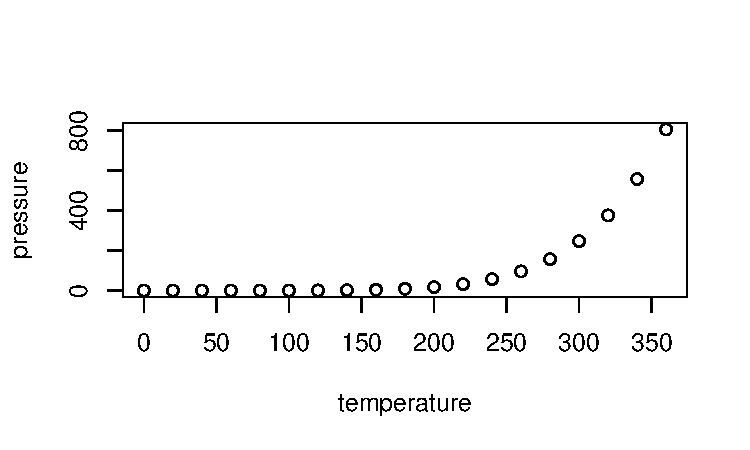
\includegraphics{thesis_files/figure-latex/pressure-1.pdf}

Note that the \texttt{echo=FALSE} parameter was added to the code chunk to prevent printing of the \textbf{R} code that generated the plot. There are plenty of other ways to add chunk options (like \texttt{fig.height} and \texttt{fig.width} in the chunk above). More information is available at \url{https://yihui.org/knitr/options/}.

Another useful chunk option is the setting of \texttt{cache=TRUE} as you see here. If document rendering becomes time consuming due to long computations or plots that are expensive to generate you can use knitr caching to improve performance. Later in this file, you'll see a way to reference plots created in \textbf{R} or external figures.

\hypertarget{loading-and-exploring-data}{%
\section{Loading and exploring data}\label{loading-and-exploring-data}}

Included in this template is a file called \texttt{flights.csv}. This file includes a subset of the larger dataset of information about all flights that departed from Seattle and Portland in 2014. More information about this dataset and its \textbf{R} package is available at \url{https://github.com/ismayc/pnwflights14}. This subset includes only Portland flights and only rows that were complete with no missing values. Merges were also done with the \texttt{airports} and \texttt{airlines} data sets in the \texttt{pnwflights14} package to get more descriptive airport and airline names.

We can load in this data set using the following commands:

The data is now stored in the data frame called \texttt{flights} in \textbf{R}. To get a better feel for the variables included in this dataset we can use a variety of functions. Here we can see the dimensions (rows by columns) and also the names of the columns.
\begin{verbatim}
[1] 12649    16
\end{verbatim}
\begin{verbatim}
 [1] "month"        "day"          "dep_time"     "dep_delay"   
 [5] "arr_time"     "arr_delay"    "carrier"      "tailnum"     
 [9] "flight"       "dest"         "air_time"     "distance"    
[13] "hour"         "minute"       "carrier_name" "dest_name"   
\end{verbatim}
Another good idea is to take a look at the dataset in table form. With this dataset having more than 20,000 rows, we won't explicitly show the results of the command here. I recommend you enter the command into the Console \textbf{\emph{after}} you have run the \textbf{R} chunks above to load the data into \textbf{R}.

While not required, it is highly recommended you use the \texttt{dplyr} package to manipulate and summarize your data set as needed. It uses a syntax that is easy to understand using chaining operations. Below I've created a few examples of using \texttt{dplyr} to get information about the Portland flights in 2014. You will also see the use of the \texttt{ggplot2} package, which produces beautiful, high-quality academic visuals.

We begin by checking to ensure that needed packages are installed and then we load them into our current working environment:

\clearpage

The example we show here does the following:
\begin{itemize}
\item
  Selects only the \texttt{carrier\_name} and \texttt{arr\_delay} from the \texttt{flights} dataset and then assigns this subset to a new variable called \texttt{flights2}.
\item
  Using \texttt{flights2}, we determine the largest arrival delay for each of the carriers.
\end{itemize}
A useful function in the \texttt{knitr} package for making nice tables in \emph{R Markdown} is called \texttt{kable}. It is much easier to use than manually entering values into a table by copying and pasting values into Excel or LaTeX. This again goes to show how nice reproducible documents can be! (Note the use of \texttt{results="asis"}, which will produce the table instead of the code to create the table.) The \texttt{caption.short} argument is used to include a shorter title to appear in the List of Tables.
\begin{longtable}[t]{lr}
\caption[Max Delays by Airline]{\label{tab:maxdelays}Maximum Delays by Airline}\\
\toprule
Airline & Max Arrival Delay\\
\midrule
Alaska Airlines Inc. & 338\\
American Airlines Inc. & 1539\\
Delta Air Lines Inc. & 371\\
Frontier Airlines Inc. & 166\\
Hawaiian Airlines Inc. & 116\\
\addlinespace
JetBlue Airways & 256\\
SkyWest Airlines Inc. & 321\\
Southwest Airlines Co. & 315\\
United Air Lines Inc. & 319\\
US Airways Inc. & 347\\
\addlinespace
Virgin America & 366\\
\bottomrule
\end{longtable}
The last two options make the table a little easier-to-read.

We can further look into the properties of the largest value here for American Airlines Inc.~To do so, we can isolate the row corresponding to the arrival delay of 1539 minutes for American in our original \texttt{flights} dataset.
\begin{verbatim}
  dep_time dep_delay arr_time tailnum flight dest air_time distance
1     1403      1553     1934  N595AA   1568  DFW      182     1616
\end{verbatim}
We see that the flight occurred on March 3rd and departed a little after 2 PM on its way to Dallas/Fort Worth. Lastly, we show how we can visualize the arrival delay of all departing flights from Portland on March 3rd against time of departure.

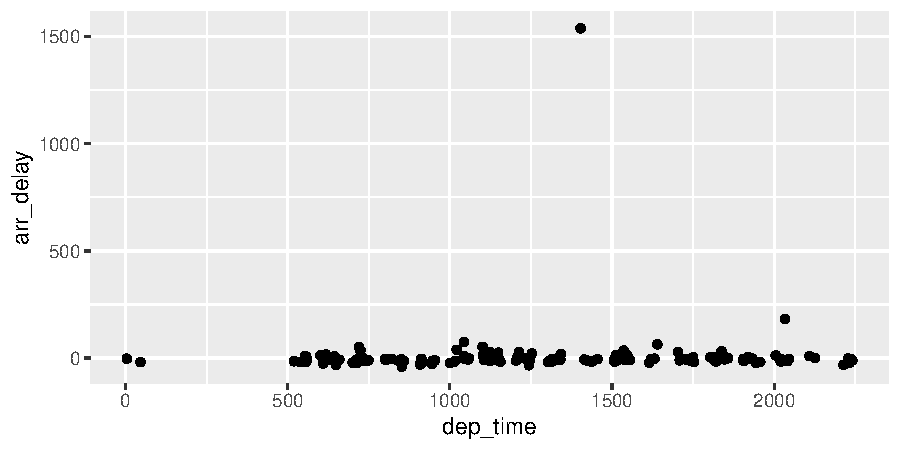
\includegraphics{thesis_files/figure-latex/march3plot-1.pdf}

\hypertarget{additional-resources}{%
\section{Additional resources}\label{additional-resources}}
\begin{itemize}
\item
  \emph{Markdown} Cheatsheet - \url{https://github.com/adam-p/markdown-here/wiki/Markdown-Cheatsheet}
\item
  \emph{R Markdown}
  \begin{itemize}
  \tightlist
  \item
    Reference Guide - \url{https://www.rstudio.com/wp-content/uploads/2015/03/rmarkdown-reference.pdf}
  \item
    Cheatsheet - \url{https://github.com/rstudio/cheatsheets/raw/master/rmarkdown-2.0.pdf}
  \end{itemize}
\item
  \emph{RStudio IDE}
  \begin{itemize}
  \tightlist
  \item
    Cheatsheet - \url{https://github.com/rstudio/cheatsheets/raw/master/rstudio-ide.pdf}
  \item
    Official website - \url{https://rstudio.com/products/rstudio/}
  \end{itemize}
\item
  Introduction to \texttt{dplyr} - \url{https://cran.rstudio.com/web/packages/dplyr/vignettes/dplyr.html}
\item
  \texttt{ggplot2}
  \begin{itemize}
  \tightlist
  \item
    Documentation - \url{https://ggplot2.tidyverse.org/}
  \item
    Cheatsheet - \url{https://github.com/rstudio/cheatsheets/raw/master/data-visualization-2.1.pdf}
  \end{itemize}
\end{itemize}
\hypertarget{math-sci}{%
\chapter{Mathematics and Science}\label{math-sci}}

\hypertarget{math}{%
\section{Math}\label{math}}

\TeX~is the best way to typeset mathematics. Donald Knuth designed \TeX~when he got frustrated at how long it was taking the typesetters to finish his book, which contained a lot of mathematics. One nice feature of \emph{R Markdown} is its ability to read LaTeX code directly.

If you are doing a thesis that will involve lots of math, you will want to read the following section which has been commented out. If you're not going to use math, skip over or delete this next commented section.

\hypertarget{chemistry-101-symbols}{%
\section{Chemistry 101: Symbols}\label{chemistry-101-symbols}}

Chemical formulas will look best if they are not italicized. Get around math mode's automatic italicizing in LaTeX by using the argument \texttt{\$\textbackslash{}mathrm\{formula\ here\}\$}, with your formula inside the curly brackets. (Notice the use of the backticks here which enclose text that acts as code.)

So, \(\mathrm{Fe_2^{2+}Cr_2O_4}\) is written \texttt{\$\textbackslash{}mathrm\{Fe\_2\^{}\{2+\}Cr\_2O\_4\}\$}.

\noindent Exponent or Superscript: \(\mathrm{O^-}\)

\noindent Subscript: \(\mathrm{CH_4}\)

To stack numbers or letters as in \(\mathrm{Fe_2^{2+}}\), the subscript is defined first, and then the superscript is defined.

\noindent Bullet: CuCl \(\bullet\) \(\mathrm{7H_{2}O}\)

\noindent Delta: \(\Delta\)

\noindent Reaction Arrows: \(\longrightarrow\) or \(\xrightarrow{solution}\)

\noindent Resonance Arrows: \(\leftrightarrow\)

\noindent Reversible Reaction Arrows: \(\rightleftharpoons\)

\hypertarget{typesetting-reactions}{%
\subsection{Typesetting reactions}\label{typesetting-reactions}}

You may wish to put your reaction in an equation environment, which means that LaTeX will place the reaction where it fits and will number the equations for you.
\begin{equation}
  \mathrm{C_6H_{12}O_6  + 6O_2} \longrightarrow \mathrm{6CO_2 + 6H_2O}
  \label{eq:reaction}
\end{equation}
We can reference this combustion of glucose reaction via Equation \eqref{eq:reaction}.

\hypertarget{other-examples-of-reactions}{%
\subsection{Other examples of reactions}\label{other-examples-of-reactions}}

\(\mathrm{NH_4Cl_{(s)}}\) \(\rightleftharpoons\) \(\mathrm{NH_{3(g)}+HCl_{(g)}}\)

\noindent \(\mathrm{MeCH_2Br + Mg}\) \(\xrightarrow[below]{above}\) \(\mathrm{MeCH_2\bullet Mg \bullet Br}\)

\hypertarget{physics}{%
\section{Physics}\label{physics}}

Many of the symbols you will need can be found on the math page \url{https://web.reed.edu/cis/help/latex/math.html} and the Comprehensive LaTeX Symbol Guide (\url{https://mirror.utexas.edu/ctan/info/symbols/comprehensive/symbols-letter.pdf}).

\hypertarget{biology}{%
\section{Biology}\label{biology}}

You will probably find the resources at \url{https://www.lecb.ncifcrf.gov/~toms/latex.html} helpful, particularly the links to bsts for various journals. You may also be interested in TeXShade for nucleotide typesetting (\url{https://homepages.uni-tuebingen.de/beitz/txe.html}). Be sure to read the proceeding chapter on graphics and tables.

\hypertarget{ref-labels}{%
\chapter{Graphics, References, and Labels}\label{ref-labels}}

\hypertarget{figures}{%
\section{Figures}\label{figures}}

If your thesis has a lot of figures, \emph{R Markdown} might behave better for you than that other word processor. One perk is that it will automatically number the figures accordingly in each chapter. You'll also be able to create a label for each figure, add a caption, and then reference the figure in a way similar to what we saw with tables earlier. If you label your figures, you can move the figures around and \emph{R Markdown} will automatically adjust the numbering for you. No need for you to remember! So that you don't have to get too far into LaTeX to do this, a couple \textbf{R} functions have been created for you to assist. You'll see their use below.

In the \textbf{R} chunk below, we will load in a picture stored as \texttt{reed.jpg} in our main directory. We then give it the caption of ``Reed logo'', the label of ``reedlogo'', and specify that this is a figure. Make note of the different \textbf{R} chunk options that are given in the R Markdown file (not shown in the knitted document).
\begin{figure}

{\centering 
\includegraphics[width=0.2\linewidth]{figure/reed} 

}

\caption{Reed logo}\label{fig:reedlogo}
\end{figure}
Here is a reference to the Reed logo: Figure \ref{fig:reedlogo}. Note the use of the \texttt{fig:} code here. By naming the \textbf{R} chunk that contains the figure, we can then reference that figure later as done in the first sentence here. We can also specify the caption for the figure via the R chunk option \texttt{fig.cap}.

\clearpage

Below we will investigate how to save the output of an \textbf{R} plot and label it in a way similar to that done above. Recall the \texttt{flights} dataset from Chapter \ref{rmd-basics}. (Note that we've shown a different way to reference a section or chapter here.) We will next explore a bar graph with the mean flight departure delays by airline from Portland for 2014.
\begin{figure}
\centering
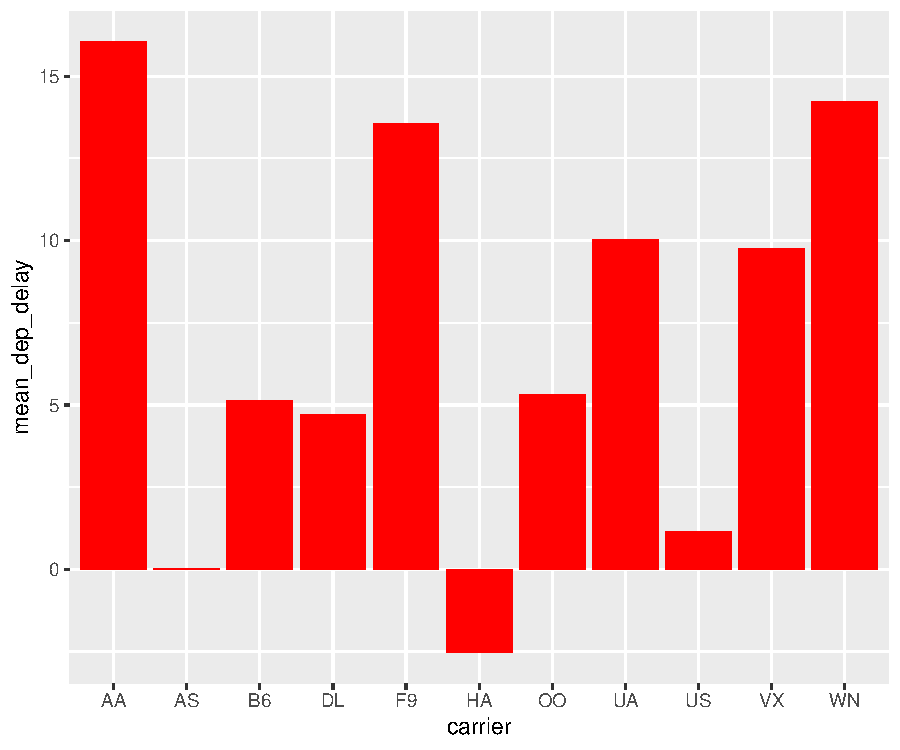
\includegraphics{thesis_files/figure-latex/delaysboxplot-1.pdf}
\caption{\label{fig:delaysboxplot}Mean Delays by Airline}
\end{figure}
Here is a reference to this image: Figure \ref{fig:delaysboxplot}.

A table linking these carrier codes to airline names is available at \url{https://github.com/ismayc/pnwflights14/blob/master/data/airlines.csv}.

\clearpage

Next, we will explore the use of the \texttt{out.extra} chunk option, which can be used to shrink or expand an image loaded from a file by specifying \texttt{"scale=\ "}. Here we use the mathematical graph stored in the ``subdivision.pdf'' file.
\begin{figure}
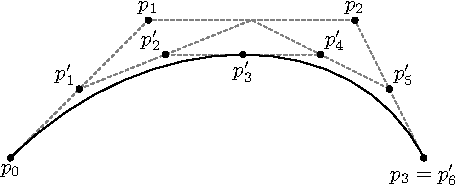
\includegraphics[scale=0.75]{figure/subdivision} \caption{Subdiv. graph}\label{fig:subd}
\end{figure}
Here is a reference to this image: Figure \ref{fig:subd}. Note that \texttt{echo=FALSE} is specified so that the \textbf{R} code is hidden in the document.

\textbf{More Figure Stuff}

Lastly, we will explore how to rotate and enlarge figures using the \texttt{out.extra} chunk option. (Currently this only works in the PDF version of the book.)
\begin{figure}
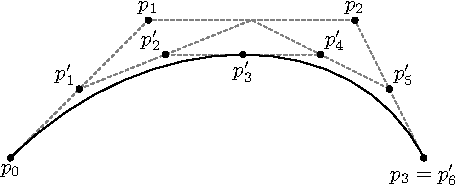
\includegraphics[angle=180, scale=1.1]{figure/subdivision} \caption{A Larger Figure, Flipped Upside Down}\label{fig:subd2}
\end{figure}
As another example, here is a reference: Figure \ref{fig:subd2}.

\hypertarget{footnotes-and-endnotes}{%
\section{Footnotes and Endnotes}\label{footnotes-and-endnotes}}

You might want to footnote something.\footnote{footnote text} The footnote will be in a smaller font and placed appropriately. Endnotes work in much the same way. More information can be found about both on the CUS site or feel free to reach out to \href{mailto:data@reed.edu}{\nolinkurl{data@reed.edu}}.

\hypertarget{bibliographies}{%
\section{Bibliographies}\label{bibliographies}}

Of course you will need to cite things, and you will probably accumulate an armful of sources. There are a variety of tools available for creating a bibliography database (stored with the .bib extension). In addition to BibTeX suggested below, you may want to consider using the free and easy-to-use tool called Zotero. The Reed librarians have created Zotero documentation at \url{https://libguides.reed.edu/citation/zotero}. In addition, a tutorial is available from Middlebury College at \url{https://sites.middlebury.edu/zoteromiddlebury/}.

\emph{R Markdown} uses \emph{pandoc} (\url{https://pandoc.org/}) to build its bibliographies. One nice caveat of this is that you won't have to do a second compile to load in references as standard LaTeX requires. To cite references in your thesis (after creating your bibliography database), place the reference name inside square brackets and precede it by the ``at'' symbol. For example, here's a reference to a book about worrying: ({\textbf{???}}). This \texttt{Molina1994} entry appears in a file called \texttt{thesis.bib} in the \texttt{bib} folder. This bibliography database file was created by a program called BibTeX. You can call this file something else if you like (look at the YAML header in the main .Rmd file) and, by default, is to placed in the \texttt{bib} folder.

For more information about BibTeX and bibliographies, see our CUS site (\url{https://web.reed.edu/cis/help/latex/index.html})\footnote{({\textbf{???}})}. There are three pages on this topic: \emph{bibtex} (which talks about using BibTeX, at \url{https://web.reed.edu/cis/help/latex/bibtex.html}), \emph{bibtexstyles} (about how to find and use the bibliography style that best suits your needs, at \url{https://web.reed.edu/cis/help/latex/bibtexstyles.html}) and \emph{bibman} (which covers how to make and maintain a bibliography by hand, without BibTeX, at \url{https://web.reed.edu/cis/help/latex/bibman.html}). The last page will not be useful unless you have only a few sources.

If you look at the YAML header at the top of the main .Rmd file you can see that we can specify the style of the bibliography by referencing the appropriate csl file. You can download a variety of different style files at \url{https://www.zotero.org/styles}. Make sure to download the file into the csl folder.

\vfill

\textbf{Tips for Bibliographies}
\begin{itemize}
\tightlist
\item
  Like with thesis formatting, the sooner you start compiling your bibliography for something as large as thesis, the better. Typing in source after source is mind-numbing enough; do you really want to do it for hours on end in late April? Think of it as procrastination.
\item
  The cite key (a citation's label) needs to be unique from the other entries.
\item
  When you have more than one author or editor, you need to separate each author's name by the word ``and'' e.g.~\texttt{Author\ =\ \{Noble,\ Sam\ and\ Youngberg,\ Jessica\},}.
\item
  Bibliographies made using BibTeX (whether manually or using a manager) accept LaTeX markup, so you can italicize and add symbols as necessary.
\item
  To force capitalization in an article title or where all lowercase is generally used, bracket the capital letter in curly braces.
\item
  You can add a Reed Thesis citation\footnote{({\textbf{???}})} option. The best way to do this is to use the phdthesis type of citation, and use the optional ``type'' field to enter ``Reed thesis'' or ``Undergraduate thesis.''
\end{itemize}
\hypertarget{anything-else}{%
\section{Anything else?}\label{anything-else}}

If you'd like to see examples of other things in this template, please contact the Data @ Reed team (email \href{mailto:data@reed.edu}{\nolinkurl{data@reed.edu}}) with your suggestions. We love to see people using \emph{R Markdown} for their theses, and are happy to help.

\hypertarget{conclusion}{%
\chapter*{Conclusion}\label{conclusion}}
\addcontentsline{toc}{chapter}{Conclusion}

If we don't want Conclusion to have a chapter number next to it, we can add the \texttt{\{-\}} attribute.

\textbf{More info}

And here's some other random info: the first paragraph after a chapter title or section head \emph{shouldn't be} indented, because indents are to tell the reader that you're starting a new paragraph. Since that's obvious after a chapter or section title, proper typesetting doesn't add an indent there.

\appendix

\hypertarget{the-first-appendix}{%
\chapter{The First Appendix}\label{the-first-appendix}}

This first appendix includes all of the R chunks of code that were hidden throughout the document (using the \texttt{include\ =\ FALSE} chunk tag) to help with readibility and/or setup.

\textbf{In the main Rmd file}
\begin{Shaded}
\begin{Highlighting}[]
\CommentTok{# This chunk ensures that the thesisdown package is}
\CommentTok{# installed and loaded. This thesisdown package includes}
\CommentTok{# the template files for the thesis.}
\ControlFlowTok{if}\NormalTok{ (}\OperatorTok{!}\KeywordTok{require}\NormalTok{(remotes)) \{}
  \ControlFlowTok{if}\NormalTok{ (params}\OperatorTok{$}\StringTok{`}\DataTypeTok{Install needed packages for \{thesisdown\}}\StringTok{`}\NormalTok{) \{}
    \KeywordTok{install.packages}\NormalTok{(}\StringTok{"remotes"}\NormalTok{, }\DataTypeTok{repos =} \StringTok{"https://cran.rstudio.com"}\NormalTok{)}
\NormalTok{  \} }\ControlFlowTok{else}\NormalTok{ \{}
    \KeywordTok{stop}\NormalTok{(}
      \KeywordTok{paste}\NormalTok{(}\StringTok{'You need to run install.packages("remotes")",}
\StringTok{            "first in the Console.'}\NormalTok{)}
\NormalTok{    )}
\NormalTok{  \}}
\NormalTok{\}}
\ControlFlowTok{if}\NormalTok{ (}\OperatorTok{!}\KeywordTok{require}\NormalTok{(thesisdown)) \{}
  \ControlFlowTok{if}\NormalTok{ (params}\OperatorTok{$}\StringTok{`}\DataTypeTok{Install needed packages for \{thesisdown\}}\StringTok{`}\NormalTok{) \{}
\NormalTok{    remotes}\OperatorTok{::}\KeywordTok{install_github}\NormalTok{(}\StringTok{"ismayc/thesisdown"}\NormalTok{)}
\NormalTok{  \} }\ControlFlowTok{else}\NormalTok{ \{}
    \KeywordTok{stop}\NormalTok{(}
      \KeywordTok{paste}\NormalTok{(}
        \StringTok{"You need to run"}\NormalTok{,}
        \StringTok{'remotes::install_github("ismayc/thesisdown")'}\NormalTok{,}
        \StringTok{"first in the Console."}
\NormalTok{      )}
\NormalTok{    )}
\NormalTok{  \}}
\NormalTok{\}}
\KeywordTok{library}\NormalTok{(thesisdown)}
\CommentTok{# Set how wide the R output will go}
\KeywordTok{options}\NormalTok{(}\DataTypeTok{width =} \DecValTok{70}\NormalTok{)}
\end{Highlighting}
\end{Shaded}
\textbf{In Chapter \ref{ref-labels}:}
\begin{Shaded}
\begin{Highlighting}[]
\CommentTok{# This chunk ensures that the thesisdown package is}
\CommentTok{# installed and loaded. This thesisdown package includes}
\CommentTok{# the template files for the thesis and also two functions}
\CommentTok{# used for labeling and referencing}
\ControlFlowTok{if}\NormalTok{ (}\OperatorTok{!}\KeywordTok{require}\NormalTok{(remotes)) \{}
  \ControlFlowTok{if}\NormalTok{ (params}\OperatorTok{$}\StringTok{`}\DataTypeTok{Install needed packages for \{thesisdown\}}\StringTok{`}\NormalTok{) \{}
    \KeywordTok{install.packages}\NormalTok{(}\StringTok{"remotes"}\NormalTok{, }\DataTypeTok{repos =} \StringTok{"https://cran.rstudio.com"}\NormalTok{)}
\NormalTok{  \} }\ControlFlowTok{else}\NormalTok{ \{}
    \KeywordTok{stop}\NormalTok{(}
      \KeywordTok{paste}\NormalTok{(}
        \StringTok{'You need to run install.packages("remotes")'}\NormalTok{,}
        \StringTok{"first in the Console."}
\NormalTok{      )}
\NormalTok{    )}
\NormalTok{  \}}
\NormalTok{\}}
\ControlFlowTok{if}\NormalTok{ (}\OperatorTok{!}\KeywordTok{require}\NormalTok{(dplyr)) \{}
  \ControlFlowTok{if}\NormalTok{ (params}\OperatorTok{$}\StringTok{`}\DataTypeTok{Install needed packages for \{thesisdown\}}\StringTok{`}\NormalTok{) \{}
    \KeywordTok{install.packages}\NormalTok{(}\StringTok{"dplyr"}\NormalTok{, }\DataTypeTok{repos =} \StringTok{"https://cran.rstudio.com"}\NormalTok{)}
\NormalTok{  \} }\ControlFlowTok{else}\NormalTok{ \{}
    \KeywordTok{stop}\NormalTok{(}
      \KeywordTok{paste}\NormalTok{(}
        \StringTok{'You need to run install.packages("dplyr")'}\NormalTok{,}
        \StringTok{"first in the Console."}
\NormalTok{      )}
\NormalTok{    )}
\NormalTok{  \}}
\NormalTok{\}}
\ControlFlowTok{if}\NormalTok{ (}\OperatorTok{!}\KeywordTok{require}\NormalTok{(ggplot2)) \{}
  \ControlFlowTok{if}\NormalTok{ (params}\OperatorTok{$}\StringTok{`}\DataTypeTok{Install needed packages for \{thesisdown\}}\StringTok{`}\NormalTok{) \{}
    \KeywordTok{install.packages}\NormalTok{(}\StringTok{"ggplot2"}\NormalTok{, }\DataTypeTok{repos =} \StringTok{"https://cran.rstudio.com"}\NormalTok{)}
\NormalTok{  \} }\ControlFlowTok{else}\NormalTok{ \{}
    \KeywordTok{stop}\NormalTok{(}
      \KeywordTok{paste}\NormalTok{(}
        \StringTok{'You need to run install.packages("ggplot2")'}\NormalTok{,}
        \StringTok{"first in the Console."}
\NormalTok{      )}
\NormalTok{    )}
\NormalTok{  \}}
\NormalTok{\}}
\ControlFlowTok{if}\NormalTok{ (}\OperatorTok{!}\KeywordTok{require}\NormalTok{(bookdown)) \{}
  \ControlFlowTok{if}\NormalTok{ (params}\OperatorTok{$}\StringTok{`}\DataTypeTok{Install needed packages for \{thesisdown\}}\StringTok{`}\NormalTok{) \{}
    \KeywordTok{install.packages}\NormalTok{(}\StringTok{"bookdown"}\NormalTok{, }\DataTypeTok{repos =} \StringTok{"https://cran.rstudio.com"}\NormalTok{)}
\NormalTok{  \} }\ControlFlowTok{else}\NormalTok{ \{}
    \KeywordTok{stop}\NormalTok{(}
      \KeywordTok{paste}\NormalTok{(}
        \StringTok{'You need to run install.packages("bookdown")'}\NormalTok{,}
        \StringTok{"first in the Console."}
\NormalTok{      )}
\NormalTok{    )}
\NormalTok{  \}}
\NormalTok{\}}
\ControlFlowTok{if}\NormalTok{ (}\OperatorTok{!}\KeywordTok{require}\NormalTok{(thesisdown)) \{}
  \ControlFlowTok{if}\NormalTok{ (params}\OperatorTok{$}\StringTok{`}\DataTypeTok{Install needed packages for \{thesisdown\}}\StringTok{`}\NormalTok{) \{}
\NormalTok{    remotes}\OperatorTok{::}\KeywordTok{install_github}\NormalTok{(}\StringTok{"ismayc/thesisdown"}\NormalTok{)}
\NormalTok{  \} }\ControlFlowTok{else}\NormalTok{ \{}
    \KeywordTok{stop}\NormalTok{(}
      \KeywordTok{paste}\NormalTok{(}
        \StringTok{"You need to run"}\NormalTok{,}
        \StringTok{'remotes::install_github("ismayc/thesisdown")'}\NormalTok{,}
        \StringTok{"first in the Console."}
\NormalTok{      )}
\NormalTok{    )}
\NormalTok{  \}}
\NormalTok{\}}
\KeywordTok{library}\NormalTok{(thesisdown)}
\KeywordTok{library}\NormalTok{(dplyr)}
\KeywordTok{library}\NormalTok{(ggplot2)}
\KeywordTok{library}\NormalTok{(knitr)}
\NormalTok{flights <-}\StringTok{ }\KeywordTok{read.csv}\NormalTok{(}\StringTok{"data/flights.csv"}\NormalTok{, }\DataTypeTok{stringsAsFactors =} \OtherTok{FALSE}\NormalTok{)}
\end{Highlighting}
\end{Shaded}
\hypertarget{the-second-appendix-for-fun}{%
\chapter{The Second Appendix, for Fun}\label{the-second-appendix-for-fun}}

\backmatter

\hypertarget{references}{%
\chapter*{References}\label{references}}
\addcontentsline{toc}{chapter}{References}

\markboth{References}{References}

\noindent

\setlength{\parindent}{-0.20in}

\hypertarget{refs}{}
\leavevmode\hypertarget{ref-aksoy2010}{}%
Aksoy, A., Dowell, D. C., \& Snyder, C. (2010). A Multicase Comparative Assessment of the Ensemble Kalman Filter for Assimilation of Radar Observations. Part II: Short-Range Ensemble Forecasts. \emph{Monthly Weather Review}, \emph{138}(4), 1273--1292. \url{http://doi.org/10.1175/2009MWR3086.1}

\leavevmode\hypertarget{ref-andersson1991}{}%
Andersson, E., Hollingsworth, A., Kelly, G., Lönnberg, P., Pailleux, J., \& Zhang, Z. (1991). Global Observing System Experiments on Operational Statistical Retrievals of Satellite Sounding Data. \emph{Monthly Weather Review}, \emph{119}(8), 1851--1865. \url{http://doi.org/10.1175/1520-0493(1991)119\%3C1851:GOSEOO\%3E2.0.CO;2}

\leavevmode\hypertarget{ref-bae2022}{}%
Bae, J.-H., \& Min, K.-H. (2022). Forecast Characteristics of Radar Data Assimilation Based on the Scales of Precipitation Systems. \emph{Remote Sensing}, \emph{14}(3, 3), 605. \url{http://doi.org/10.3390/rs14030605}

\leavevmode\hypertarget{ref-chang2017}{}%
Chang, W., Jacques, D., Fillion, L., \& Baek, S.-J. (2017). Assimilation of Hourly Surface Observations with the Canadian High-Resolution Ensemble Kalman Filter. \emph{Atmosphere-Ocean}, \emph{55}(4-5), 247--263. \url{http://doi.org/10.1080/07055900.2017.1384361}

\leavevmode\hypertarget{ref-chen2016}{}%
Chen, X., Zhao, K., Sun, J., Zhou, B., \& Lee, W.-C. (2016). Assimilating surface observations in a four-dimensional variational Doppler radar data assimilation system to improve the analysis and forecast of a squall line case. \emph{Advances in Atmospheric Sciences}, \emph{33}(10), 1106--1119. \url{http://doi.org/10.1007/s00376-016-5290-0}

\leavevmode\hypertarget{ref-cherubini2006}{}%
Cherubini, T., Businger, S., Velden, C., \& Ogasawara, R. (2006). The Impact of Satellite-Derived Atmospheric Motion Vectors on Mesoscale Forecasts over Hawaii. \emph{Monthly Weather Review}, \emph{134}(7), 2009--2020. \url{http://doi.org/10.1175/MWR3163.1}

\leavevmode\hypertarget{ref-clark2009}{}%
Clark, A. J., Gallus, W. A., Xue, M., \& Kong, F. (2009). A Comparison of Precipitation Forecast Skill between Small Convection-Allowing and Large Convection-Parameterizing Ensembles. \emph{Weather and Forecasting}, \emph{24}(4), 1121--1140. \url{http://doi.org/10.1175/2009WAF2222222.1}

\leavevmode\hypertarget{ref-dillon2021}{}%
Dillon, M. E., Maldonado, P., Corrales, P., Skabar, Y. G., Ruiz, J., Sacco, M., \ldots{} Miyoshi, T. (2021). A rapid refresh ensemble based data assimilation and forecast system for the RELAMPAGO field campaign. \emph{Atmospheric Research}, 105858. \url{http://doi.org/10.1016/j.atmosres.2021.105858}

\leavevmode\hypertarget{ref-eyre2022}{}%
Eyre, J. R., Bell, W., Cotton, J., English, S. J., Forsythe, M., Healy, S. B., \& Pavelin, E. G. (2022). Assimilation of satellite data in numerical weather prediction. Part II: Recent years. \emph{Quarterly Journal of the Royal Meteorological Society}, \emph{148}(743), 521--556. \url{http://doi.org/10.1002/qj.4228}

\leavevmode\hypertarget{ref-eyre2020}{}%
Eyre, J. R., English, S. J., \& Forsythe, M. (2020). Assimilation of satellite data in numerical weather prediction. Part I: The early years. \emph{Quarterly Journal of the Royal Meteorological Society}, \emph{146}(726), 49--68. \url{http://doi.org/10.1002/qj.3654}

\leavevmode\hypertarget{ref-gasperoni2018}{}%
Gasperoni, N. A., Wang, X., Brewster, K. A., \& Carr, F. H. (2018). Assessing Impacts of the High-Frequency Assimilation of Surface Observations for the Forecast of Convection Initiation on 3 April 2014 within the Dallas--Fort Worth Test Bed. \emph{Monthly Weather Review}, \emph{146}(11), 3845--3872. \url{http://doi.org/10.1175/MWR-D-18-0177.1}

\leavevmode\hypertarget{ref-ha2014}{}%
Ha, S.-Y., \& Snyder, C. (2014). Influence of Surface Observations in Mesoscale Data Assimilation Using an Ensemble Kalman Filter. \emph{Monthly Weather Review}, \emph{142}(4), 1489--1508. \url{http://doi.org/10.1175/MWR-D-13-00108.1}

\leavevmode\hypertarget{ref-kalnay2002}{}%
Kalnay, E. (2002, November 6). Atmospheric Modeling, Data Assimilation and Predictability. \url{http://doi.org/10.1017/CBO9780511802270}

\leavevmode\hypertarget{ref-kelly1978}{}%
Kelly, G. a. M., Mills, G. A., \& Smith, W. L. (1978). Impact of Nimbus-6 Temperature Soundings on Australian Region Forecasts. \emph{Bulletin of the American Meteorological Society}, \emph{59}(4), 393--406. \url{http://doi.org/10.1175/1520-0477-59.4.393}

\leavevmode\hypertarget{ref-maejima2019}{}%
Maejima, Y., Miyoshi, T., Kunii, M., Seko, H., \& Sato, K. (2019). Impact of Dense and Frequent Surface Observations on 1-Minute-Update Severe Rainstorm Prediction: A Simulation Study. \emph{Journal of the Meteorological Society of Japan. Ser. II}, \emph{97}(1), 253--273. \url{http://doi.org/10.2151/jmsj.2019-014}

\leavevmode\hypertarget{ref-ohring1979}{}%
Ohring, G. (1979). Impact of Satellite Temperature Sounding Data on Weather Forecasts. \emph{Bulletin of the American Meteorological Society}, \emph{60}(10), 1142--1147. \url{http://doi.org/10.1175/1520-0477(1979)060\%3C1142:IOSTSD\%3E2.0.CO;2}

\leavevmode\hypertarget{ref-sawada2019}{}%
Sawada, M., Ma, Z., Mehra, A., Tallapragada, V., Oyama, R., \& Shimoji, K. (2019). Impacts of Assimilating High-Resolution Atmospheric Motion Vectors Derived from Himawari-8 on Tropical Cyclone Forecast in HWRF. \emph{Monthly Weather Review}, \emph{147}(10), 3721--3740. \url{http://doi.org/10.1175/MWR-D-18-0261.1}

\leavevmode\hypertarget{ref-sobash2015}{}%
Sobash, R. A., \& Stensrud, D. J. (2015). Assimilating Surface Mesonet Observations with the EnKF to Improve Ensemble Forecasts of Convection Initiation on 29 May 2012. \emph{Monthly Weather Review}, \emph{143}(9), 3700--3725. \url{http://doi.org/10.1175/MWR-D-14-00126.1}

\leavevmode\hypertarget{ref-stensrud2013}{}%
Stensrud, D. J., Wicker, L. J., Xue, M., Dawson, D. T., Yussouf, N., Wheatley, D. M., \ldots{} Brewster, K. A. (2013). Progress and challenges with Warn-on-Forecast. \emph{Atmospheric Research}, \emph{123}, 2--16. \url{http://doi.org/10.1016/j.atmosres.2012.04.004}

\leavevmode\hypertarget{ref-wheatley2010}{}%
Wheatley, D. M., \& Stensrud, D. J. (2010). The Impact of Assimilating Surface Pressure Observations on Severe Weather Events in a WRF Mesoscale Ensemble System. \emph{Monthly Weather Review}, \emph{138}(5), 1673--1694. \url{http://doi.org/10.1175/2009MWR3042.1}

\leavevmode\hypertarget{ref-whitaker2008}{}%
Whitaker, J. S., Hamill, T. M., Wei, X., Song, Y., \& Toth, Z. (2008). Ensemble Data Assimilation with the NCEP Global Forecast System. \emph{Monthly Weather Review}, \emph{136}(2), 463--482. \url{http://doi.org/10.1175/2007MWR2018.1}

\leavevmode\hypertarget{ref-wu2014}{}%
Wu, T.-C., Liu, H., Majumdar, S. J., Velden, C. S., \& Anderson, J. L. (2014). Influence of Assimilating Satellite-Derived Atmospheric Motion Vector Observations on Numerical Analyses and Forecasts of Tropical Cyclone Track and Intensity. \emph{Monthly Weather Review}, \emph{142}(1), 49--71. \url{http://doi.org/10.1175/MWR-D-13-00023.1}


% Index?

\end{document}
